%! Author = Kevin Lin
%! Date = 10/23/2025

% Preamble
\documentclass[11pt,a4paper,margin=1in]{article}

% Packages
\usepackage{graphicx}
\usepackage{float}
\usepackage{amsmath}
\usepackage{amssymb}
\usepackage{enumerate}

\usepackage{lipsum}

\usepackage{listings}
\usepackage{soul}
\usepackage{color}

\definecolor{codegreen}{rgb}{0,0.6,0}
\definecolor{codegray}{rgb}{0.5,0.5,0.5}
\definecolor{codepurple}{rgb}{0.58,0,0.82}
\definecolor{backcolour}{rgb}{0.95,0.95,0.92}

\lstdefinestyle{mystyle}{
	backgroundcolor=\color{backcolour},   
	commentstyle=\color{codegreen},
	keywordstyle=\color{magenta},
	numberstyle=\tiny\color{codegray},
	stringstyle=\color{codepurple},
	basicstyle=\footnotesize,
	breakatwhitespace=false,         
	breaklines=true,                 
	captionpos=b,                    
	keepspaces=true,                 
	numbers=left,                    
	numbersep=5pt,                  
	showspaces=false,                
	showstringspaces=false,
	showtabs=false,                  
	tabsize=2
}

\lstset{style=mystyle}

\title{HW 2}
\author{Kevin Lin}
\date{10/23/2025}

% Document
\begin{document}
\maketitle
\section{}
    Define deviation $D = E[(X - c)^2]$ for some constant $c$. We want to find
    the value of $c$ that minimizes $D$. We can expand $D$ as follows:
    \begin{gather*}
        D = E[(X - c)^2] = E[X^2 - 2cX + c^2] = E[X^2] - 2cE[X] + c^2
    \end{gather*}
    To find the minimum value of $D$, we can take the derivative of $D$
    with respect to $c$ and set it equal to 0:
    \begin{gather*}
        \frac{dD}{dc} = -2E[X] + 2c = 0 \therefore c = E[X]
    \end{gather*}
    Thus, the $D$ is minimized when $c = E[X]$.

\section{}
    Note that each jump is independent and identically distributed. For the current
    particle's current position $k$, it can either hop left or right with probability
    $p$ and $1 - p$ respectively. Thus, we can express the expected position $E[X_n]$
    after $n$ jumps as follows:
    \begin{gather*}
        E[X_n] = \sum_{k=1}^n E[X_k] = nE[X_k] \\
        E[X_k] = (-1)p + (1)(1 - p) = 1 - 2p \\
        \therefore E[X_n] = n(1 - 2p)
    \end{gather*}

    Likewise, we can calculate the variance $Var(X_n)$ as:
    \begin{gather*}
        Var(X_n) = \sum_{k=1}^n Var(X_k) = nVar(X_k) \\
        Var(X_k) = E[X_k^2] - (E[X_k])^2 \\ 
        E[X_k^2] = (-1)^2p + (1)^2(1 - p) = 1 \\
        Var(X_k) = 1 - (1 - 2p)^2 = 4p(1 - p) \\
        \therefore Var(X_n) = 4np(1 - p)
    \end{gather*}

\section{}
\begin{lstlisting}[language=python]
import numpy as np
import matplotlib.pyplot as plt
from scipy.stats import norm

np.random.seed(0)

X_bar_n = np.mean(np.random.uniform(0, 1, 100))
mu_X = 0.5
var_X_bar = (1/12)/100
std_X_bar = np.sqrt(var_X_bar)
print("Mean:", mu_X)
print("Var:", var_X_bar)

a_vals = [-2, -1, -0.5, -0.25, 0, 0.25, 0.5, 1, 2]
z_vals = []
for _ in range(100):
    sample_mean = np.mean(np.random.uniform(0, 1, 100))
    z_vals.append((sample_mean - mu_X) / np.sqrt(var_X / 100))

counts = [int((np.array(z_vals) <= a).sum()) for a in a_vals]
cdf = 100 * norm.cdf(a_vals)

plt.plot(a_vals, counts, "o-", label="Counts Zn <= a")
plt.plot(a_vals, cdf, "s--", label="100x CDF (N(0,1))")
plt.legend()
plt.xlabel("a values")
plt.ylabel("Counts / 100x CDF")
plt.show()
\end{lstlisting}
\begin{verbatim}
Mean: 0.5
Var: 0.0008333333333333333
\end{verbatim}
\begin{figure}[H]
    \centering
    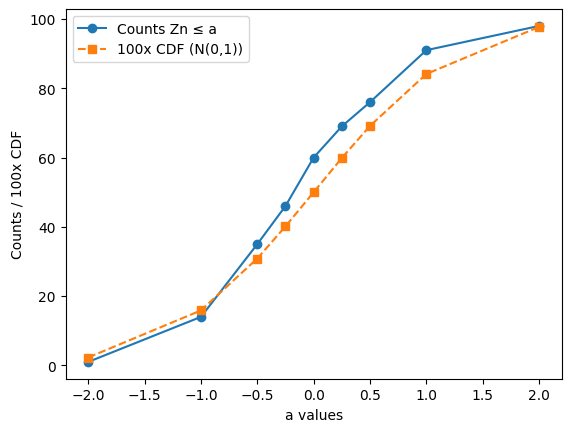
\includegraphics[width=0.8\textwidth]{3.png}
\end{figure}

\section{}
\begin{lstlisting}[language=python]
import numpy as np
import matplotlib.pyplot as plt

np.random.seed(0)

Xbars_normal = []
Xbars_cauchy = []
for i in range(1000):
    Xbars_normal.append(np.mean(np.random.standard_normal(size=i + 1)))
    Xbars_cauchy.append(np.mean(np.random.standard_cauchy(size=i + 1)))

def plot(Xbars, title):
    plt.plot(range(1, 1001), Xbars)
    plt.xlabel("n")
    plt.ylabel("Sample Mean")
    plt.title(title)
    plt.show()

plot(Xbars_normal, "Sample Means from Standard Normal Distribution")
plot(Xbars_cauchy, "Sample Means from Standard Cauchy Distribution")
\end{lstlisting}
\begin{figure}[H]
    \centering
    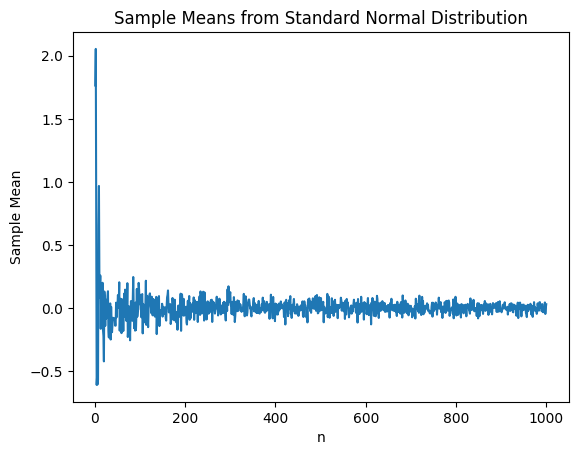
\includegraphics[width=0.8\textwidth]{4norm.png}
\end{figure}
\begin{figure}[H]
    \centering
    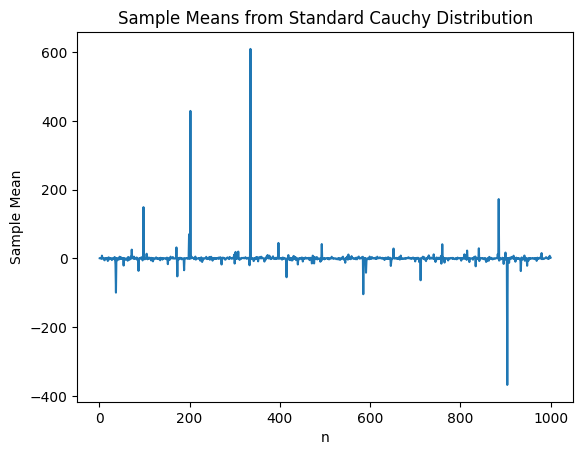
\includegraphics[width=0.8\textwidth]{4cauchy.png}
\end{figure}

    \noindent The Cauchy distribution of sample means differs from the normal distribution as 
    the Cauchy distribution has no finite mean (expectation is undefined). Note:

    \begin{align*}
        E[X] &= \int_{-\infty}^{\infty} x f_X(x) dx = \int_{-\infty}^{\infty} \frac{x}{\pi(1 + x^2)} dx \\
        &\approx \int_{-\infty}^{\infty} \frac{1}{x} dx = \text{undefined}
    \end{align*}
\end{document}